%\documentclass[conference]{IEEEtran}

%\usepackage{amsmath,amssymb,amsfonts}
%\usepackage{algorithmic}
%\usepackage{graphicx}
%\usepackage{textcomp}
%\usepackage{xcolor}

%\usepackage[sorting=none,doi=false,isbn=false,url=false,eprint=false, giveninits=true]{biblatex}
%\AtBeginBibliography{\footnotesize}
%\addbibresource{refs.bib}

\documentclass[conference, a4paper]{IEEEtran}  % Added a4paper option

\usepackage{amsmath,amssymb,amsfonts}
\usepackage{algorithmic}
\usepackage{graphicx}
\usepackage{textcomp}
\usepackage{xcolor}

% Add geometry package for precise A4 formatting
\usepackage[pass]{geometry}  % Preserves IEEE margins
\geometry{a4paper, margin=1in}  % Explicit A4 with 1-inch margins

\usepackage[backend=bibtex, sorting=none,doi=false,isbn=false,url=false,eprint=false, giveninits=true]{biblatex}
\AtBeginBibliography{\footnotesize}
\addbibresource{refs.bib}


\begin{document}


\title{Physics-Informed Neural Networks for Anisotropic Cardiac Activation Mapping}

\author{
\IEEEauthorblockN{Mohamed A. M. Gad}
\IEEEauthorblockA{\textit{Dept. of Systems and Biomedical Engineering} \\
\textit{Faculty of Engineering, Cairo University}\\
Giza, Egypt \\
mohamed.a.gad@outlook.com}
\and
\IEEEauthorblockN{Sherif M. M. El-Gendy}
\IEEEauthorblockA{\textit{Dept. of Systems and Biomedical Engineering} \\
\textit{Faculty of Engineering, Cairo University}\\
Giza, Egypt \\
sherif.gendy04@eng-st.cu.edu.eg}
\and
\IEEEauthorblockN{Mazen A. A. Atlam}
\IEEEauthorblockA{\textit{Dept. of Systems and Biomedical Engineering} \\
\textit{Faculty of Engineering, Cairo University}\\
Giza, Egypt \\
mazen.atlam04@eng-st.cu.edu.eg}
\and
\IEEEauthorblockN{Ahmed S.A. Mohamed}
\IEEEauthorblockA{\textit{\textsuperscript{1}Eng. Math Dept., Faculty of Engineering, Cairo University} \\
\textit{\textsuperscript{2}University of Science and Technology, Zewail City}\\
Giza, Egypt \\
aashiry@ieee.org, ORCID: 0000-0002-9895-5723}
}

\maketitle

\begin{abstract}
Cardiac activation mapping is critical for guiding catheter ablation of arrhythmias but remains challenging due to the difficulty of reconstructing wavefront propagation from sparse intracardiac catheter scans. Existing methods often neglect the physical laws governing electrical signal propagation in cardiac tissues. Approaches that do incorporate physics rely on isotropic models, assuming constant conduction velocity in all directions, and thus fail to account for the influence of fiber orientation, leading to physiologically inconsistent activation maps. In this article, we propose a novel Physics-Informed Neural Network (PINN) framework for cardiac activation mapping that directly incorporates the anisotropic Eikonal equation into the learning process. This formulation embeds the underlying physics of cardiac conduction and explicitly models the effect of myocardial fiber orientation on wavefront propagation. The framework employs a dual-network architecture: one network estimates activation time $\phi(\mathbf{x})$, and the other reconstructs the direction-dependent conduction velocity tensor $\mathbf{D}(\mathbf{x})$ from sparse intracardiac catheter data. Evaluated on a dataset with sharp conductivity transitions, the framework accurately reconstructed activation times (NRMSE: 1.12\%) and captured key features of conduction anisotropy. This physics-consistent approach represents a significant step toward clinically reliable cardiac activation maps for ablation planning.
\end{abstract}

\begin{IEEEkeywords}
Cardiac Electrophysiology, Activation Mapping, Physics-Informed Neural Networks (PINNs), Eikonal Equation, Catheter Ablation, Heart Arrhythmia.
\end{IEEEkeywords}

\section{Introduction}

Cardiac arrhythmias represent a major global health burden, affecting over 59 million people worldwide and contributing significantly to cardiovascular morbidity and mortality \cite{roth2020}. Among these, atrial fibrillation (AF) is the most prevalent sustained arrhythmia, impacting millions of people all over the world. For example, in the US alone, 2.7–6.1 million Americans suffer from atrial fibrillation, with projections suggesting this number could rise to 12.1 million by 2030 \cite{roth2020, Colilla2013}. Ventricular arrhythmias like tachycardia (VT) affect around 300,000 patients annually in the US and account for 50\% of cardiovascular deaths \cite{AlKhatib2018}. Catheter ablation has become a cornerstone therapy for these conditions, with more than 500,000 procedures performed globally each year to disrupt abnormal electrical pathways \cite{Calkins2017}. The efficacy of ablation critically depends on accurate cardiac activation mapping, where clinicians record local activation times (LATs) at discrete cardiac sites using catheter electrodes.

Cardiac activation maps integrate LATs into a spatiotemporal representation of electrical wavefront propagation, delineating the sequence of myocardial depolarization through isochronal contours (lines of equal activation time) \cite{DURRER1970}. Conduction velocity (CV), derived from the spatial gradient of LATs, quantifies the speed (m/s) and direction of wavefront movement \cite{ColliFranzone1998}. Critically, myocardial tissue exhibits electrical anisotropy, wherein CV is heavily influenced by the orientation of cardiac fibers relative to the wavefront direction \cite{Spach1981}. CV is typically 2–3 times faster when propagation occurs parallel to fiber orientation (longitudinal direction) compared to perpendicular (transverse direction) due to higher intercellular coupling via gap junctions along fiber axes \cite{Spach1981,KLBER2004}. Consequently, activation maps must account for fiber orientation to avoid misinterpretation of conduction properties, as wavefronts traversing transverse to fibers may mimic pathological slowing or conduction block, even in healthy tissue \cite{Spach1981,Taccardi1994}.


\section{Previous Work}

The reconstruction of cardiac activation maps from sparse intracardiac catheter data has evolved from simple interpolation methods to more advanced machine learning (ML) techniques, and most recently to physics-informed models. Early efforts used interpolation strategies such as radial basis functions (RBFs) and cosine-fit methods \cite{Mase2010} to estimate activation and conduction velocity maps. While computationally efficient, these methods failed to incorporate the underlying physics of electrophysiological wave propagation, making them unreliable for capturing nontrivial patterns such as curved or broken wavefronts.

To enhance robustness and handle uncertainty, later approaches adopted statistical models. Coveney et al. \cite{coveney2020} introduced a Gaussian Process-based probabilistic interpolation method that provided activation time estimates along with uncertainty quantification—an advantage in low-resolution or noisy scenarios. However, like geometric methods, these statistical models lacked any enforcement of physical laws, potentially leading to physiologically implausible predictions that violate known constraints of cardiac conduction.

To overcome these issues, supervised ML models were developed to directly learn mappings from electroanatomical data. Architectures such as SATDNN-AT and DirectMap \cite{Karoui2021} improved predictive accuracy and robustness in sparse data conditions. Yet, they do not enforce biophysical consistency and can produce activation maps that are visually plausible but physically invalid. Without explicitly embedding conduction physics, such models risk generating activation patterns that contradict the known dynamics of wavefront propagation in cardiac tissue.

Physics-Informed Neural Networks (PINNs) offer a hybrid solution by integrating mechanistic modeling with data-driven learning \cite{raissi2019}. Sahli Costabal et al. \cite{SahliCostabal2020} applied this approach by incorporating the isotropic Eikonal equation into a PINN framework, enabling simultaneous inference of activation times and scalar conduction velocity fields. By embedding the governing physics into the learning process, their model achieved improved accuracy, stability, and sample efficiency. However, a key limitation remains: the assumption of isotropic conduction ignores the directional dependence introduced by cardiac fiber architecture. Such models treat conduction velocity as uniform in all directions, neglecting the anisotropy that plays a central role in physiological and pathological activation dynamics.

Building on these advances, our work represents the natural evolution of cardiac activation mapping by extending the PINN framework to incorporate anisotropic conduction. Specifically, we integrate the anisotropic Eikonal equation \cite{ColliFranzone1990} directly into the learning process, enabling the model to account for the direction-dependent effects of myocardial fiber orientation, an aspect overlooked in previous PINN-based approaches that assumed isotropic conduction.

\section{Methodology}

Physics-Informed Neural Networks (PINNs) represent a recent advancement in machine learning for solving inverse problems constrained by partial differential equations (PDEs) \cite{raissi2019,karniadakis2021physics}. By integrating the underlying physics into the neural network's loss function, PINNs can accurately reconstruct complex dynamical systems even when available data is sparse. Unlike conventional neural networks that rely heavily on large volumes of labeled data, PINNs leverage domain knowledge in the form of PDEs, enabling faster and more physically consistent learning \cite{cuomo2022scientific,mao2020physics}.

The anisotropic Eikonal equation provides a mathematical model for simulating electrical activation in cardiac tissue, explicitly accounting for the direction-dependent effects of fiber orientation on wavefront propagation \cite{ColliFranzone1990, Grandits2021Springer}. We integrate this equation into the proposed PINN framework as the governing physical constraint embedded within the learning process.

The anisotropic Eikonal equation governs the activation time $\phi(\mathbf{x})$ at each spatial location $\mathbf{x}$ as follows \cite{Grandits2021Springer}:
\begin{equation}
    \sqrt{ \mathbf{D}(\mathbf{x}) \nabla \phi(\mathbf{x}) \cdot \nabla  \phi(\mathbf{x})} = 1
\end{equation}
where $\mathbf{D}(\mathbf{x})$ is the local conduction velocity tensor that encodes directional variations in wavefront speed due to underlying myocardial fiber architecture. Unlike isotropic models that assume uniform conduction in all directions, this anisotropic formulation enables the model to capture direction-dependent conduction patterns—crucial for physiologically accurate activation maps.

To infer activation times and conduction velocity tensors from sparse intracardiac catheter data, we utilize a dual-network PINN architecture. One network approximates the activation time $\phi(\mathbf{x})$, while the other approximates the conduction velocity tensor $\mathbf{D}(\mathbf{x})$, as shown in Fig. \ref{fig:NNArch}, ensuring that the solution remains consistent with the anisotropic Eikonal equation.

\begin{figure}
    \centering
    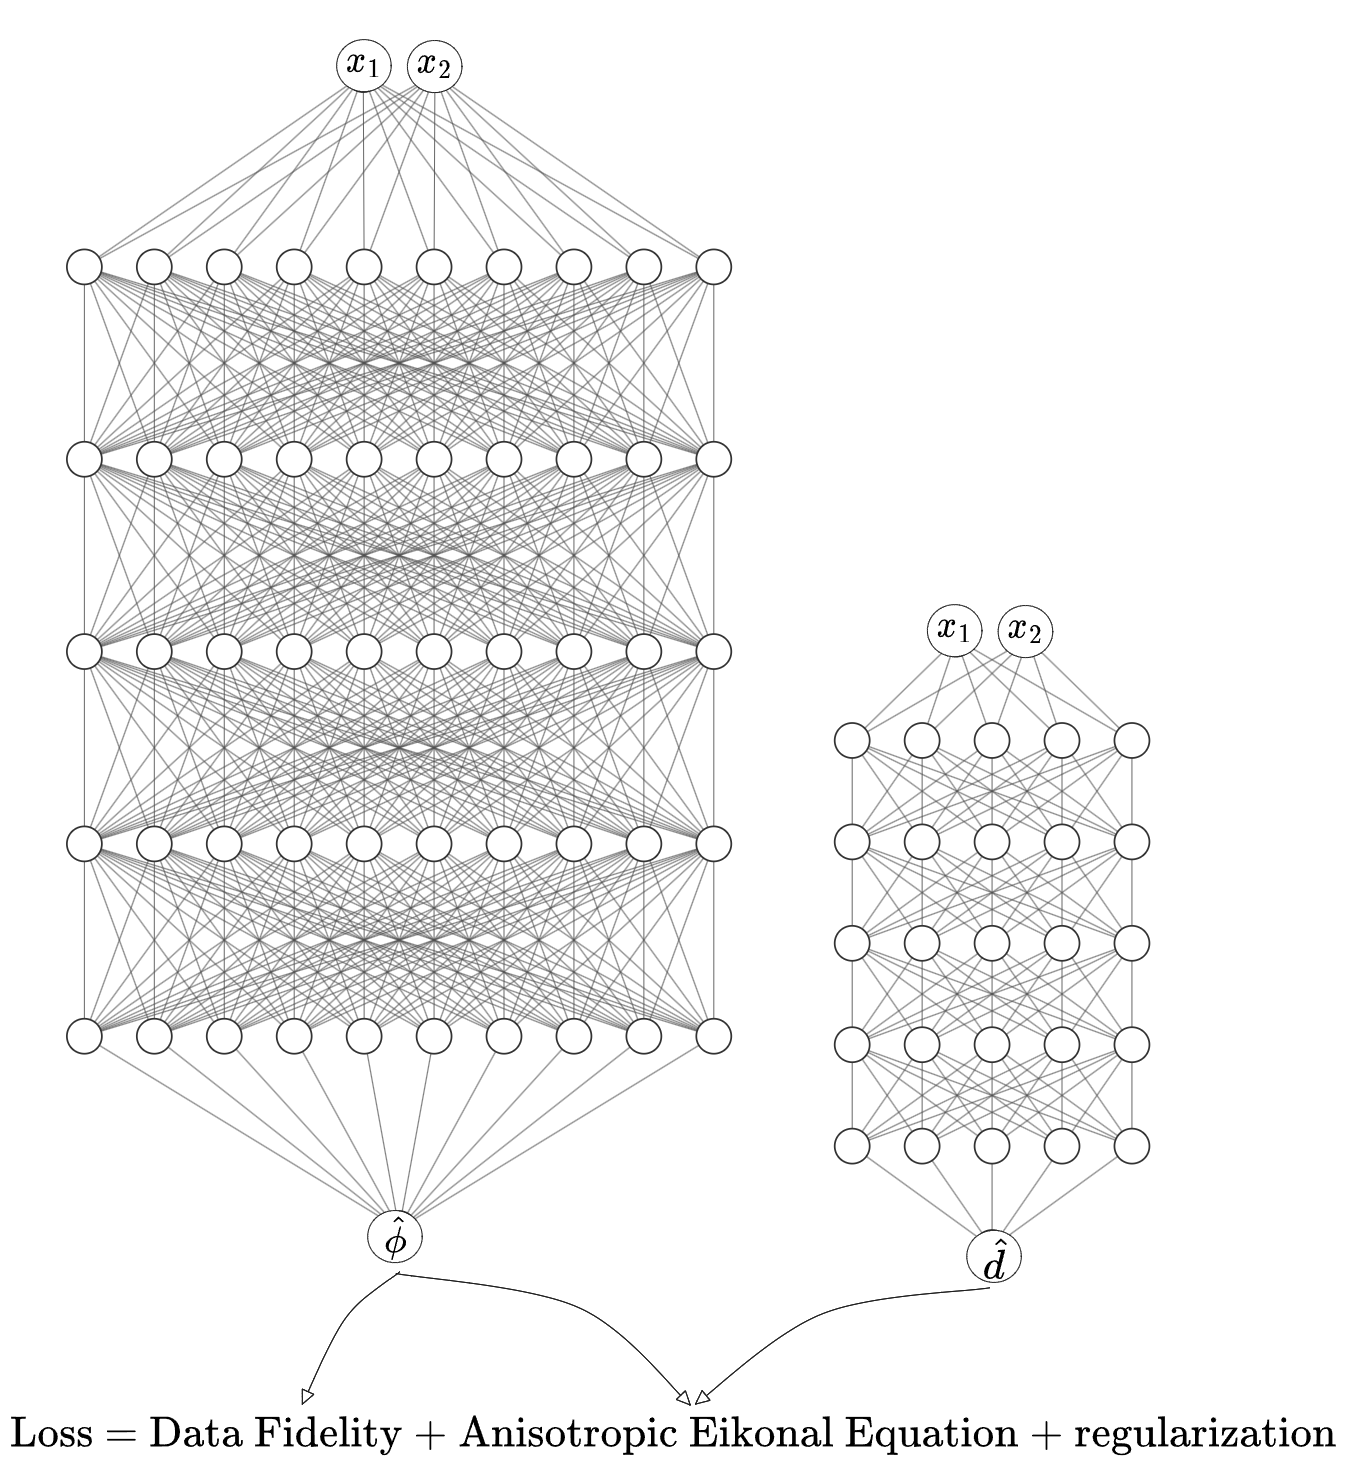
\includegraphics[width=1\linewidth]{figures/NeuralNet.png}
    \caption{
    Schematic representation of the physics-informed neural network architecture used in this study. The framework consists of two neural networks: one network estimates the conduction velocity tensor field (right neural network), while the other predicts the activation time across the spatial domain (left neural network).
    }
    \label{fig:NNArch}
\end{figure}

\subsection{Neural Networks Architecture}


\textbf{Activation Time Network} ($\text{NN}_\phi$): The first neural network, composed of five hidden layers with ten neurons per layer and parameterized by $\theta_\phi$, approximates a scalar activation time given 2D spatial input coordinates $\mathbf{x}$.
\begin{equation}
\hat{\phi}(\mathbf{x}) := \text{NN}_\phi(\mathbf{x}; \theta_\phi)
\end{equation}

\textbf{Velocity Tensor Network} ($\text{NN}_D$): The second neural network, parameterized by $\theta_D$, consists of five hidden layers with five neurons each. It maps the spatial coordinates $\mathbf{x}$ to a set of intermediate parameters that define a symmetric and positive-definite conduction velocity tensor. We denote this parameter set as $\mathbf{d}(\mathbf{x})$, where

\begin{equation}
    \mathbf{d}(\mathbf{x}) = [e_1(\mathbf{x}), e_2(\mathbf{x}), a(\mathbf{x})],
\end{equation}

with $e_1$ and $e_2$ representing the squared conduction speeds along the longitudinal and transverse fiber directions, respectively, and $a$ denoting the local fiber orientation angle. The network output is defined as

\begin{equation}
    \hat{\mathbf{d}}(\mathbf{x}) := \text{NN}_D(\mathbf{x}; \theta_D).
\end{equation}

To reconstruct the conduction velocity tensor $\mathbf{D}(\mathbf{x})$, we rotate the diagonal tensor composed of $e_1$ and $e_2$ using the fiber orientation angle $a(\mathbf{x})$ \cite{Arsigny2007}:

\begin{equation}
\mathbf{D}(\mathbf{x}) = R(a(\mathbf{x}))^\top 
\begin{bmatrix}
e_1(\mathbf{x}) & 0 \\
0 & e_2(\mathbf{x})
\end{bmatrix}
R(a(\mathbf{x}))
\end{equation}

where the 2D rotation matrix $R(a)$ is given by:
\begin{equation}
R(a) = 
\begin{bmatrix}
\cos a & -\sin a \\
\sin a & \cos a
\end{bmatrix}
\end{equation}

\subsection{Loss Function and Optimization}

The training objective is defined as a composite loss:
\begin{equation}
\mathcal{L}(\theta_\phi, \theta_D) = \mathcal{L}_{\text{data}} + \alpha_{\text{eiko}} \mathcal{L}_{\text{eiko}} + \alpha_{\text{reg}} \mathcal{L}_{\text{reg}}
\end{equation}

\textbf{Data Loss} ($\mathcal{L}_{\text{data}}$): Penalizes deviation from observed activation times at known $N_d$ data points:
\begin{equation}
\mathcal{L}_{\text{data}} = \frac{1}{N_d} \sum_{i=1}^{N_d} \left(\hat{\phi}(\mathbf{x}_i) - \phi(\mathbf{x}_i)\right)^2
\end{equation}

\textbf{Eikonal Residual Loss} ($\mathcal{L}_{\text{eiko}}$): Enforces satisfaction of the anisotropic Eikonal equation at $N_c$ collocation points:
\begin{equation}
    \mathcal{L}_{\text{eiko}} = \frac{1}{N_c} \sum_{j=1}^{N_c} \left(\sqrt{ \mathbf{\hat D}(\mathbf{x}_j) \nabla \hat{\phi}(\mathbf{x}_j) \cdot \nabla \hat{\phi}(\mathbf{x}_j)} - 1\right)^2
\end{equation}


\textbf{Regularization Loss} ($\mathcal{L}_{\text{reg}}$): To encourage spatial regularity, we incorporate Huber total variation $\left(\text{TV}_{\text{Huber}}\right)$ as a penalization term, as it has been demonstrated to favor piecewise constant structures in the estimated fields \cite{Chambolle_Pock_2016}.
\begin{equation}
    \mathcal{L}_{\text{reg}} = \sum_{k \in \{e_1, e_2, a\}} \text{TV}_{\text{Huber}}(k(\mathbf{x}))
\end{equation}


This formulation enables physically consistent inference of activation patterns while explicitly modeling the impact of fiber orientation, a critical determinant of wavefront propagation in realistic cardiac tissue.

The proposed framework is implemented in TensorFlow \cite{abadi2016tensorflowlargescalemachinelearning}. The neural networks are trained by minimizing the total loss function using the ADAM optimizer \cite{kingma2017adammethodstochasticoptimization}, thereby learning the parameters $\theta_\phi$ and $\theta_D$.

\section{Results and Discussion}
\begin{figure}
    \centering
    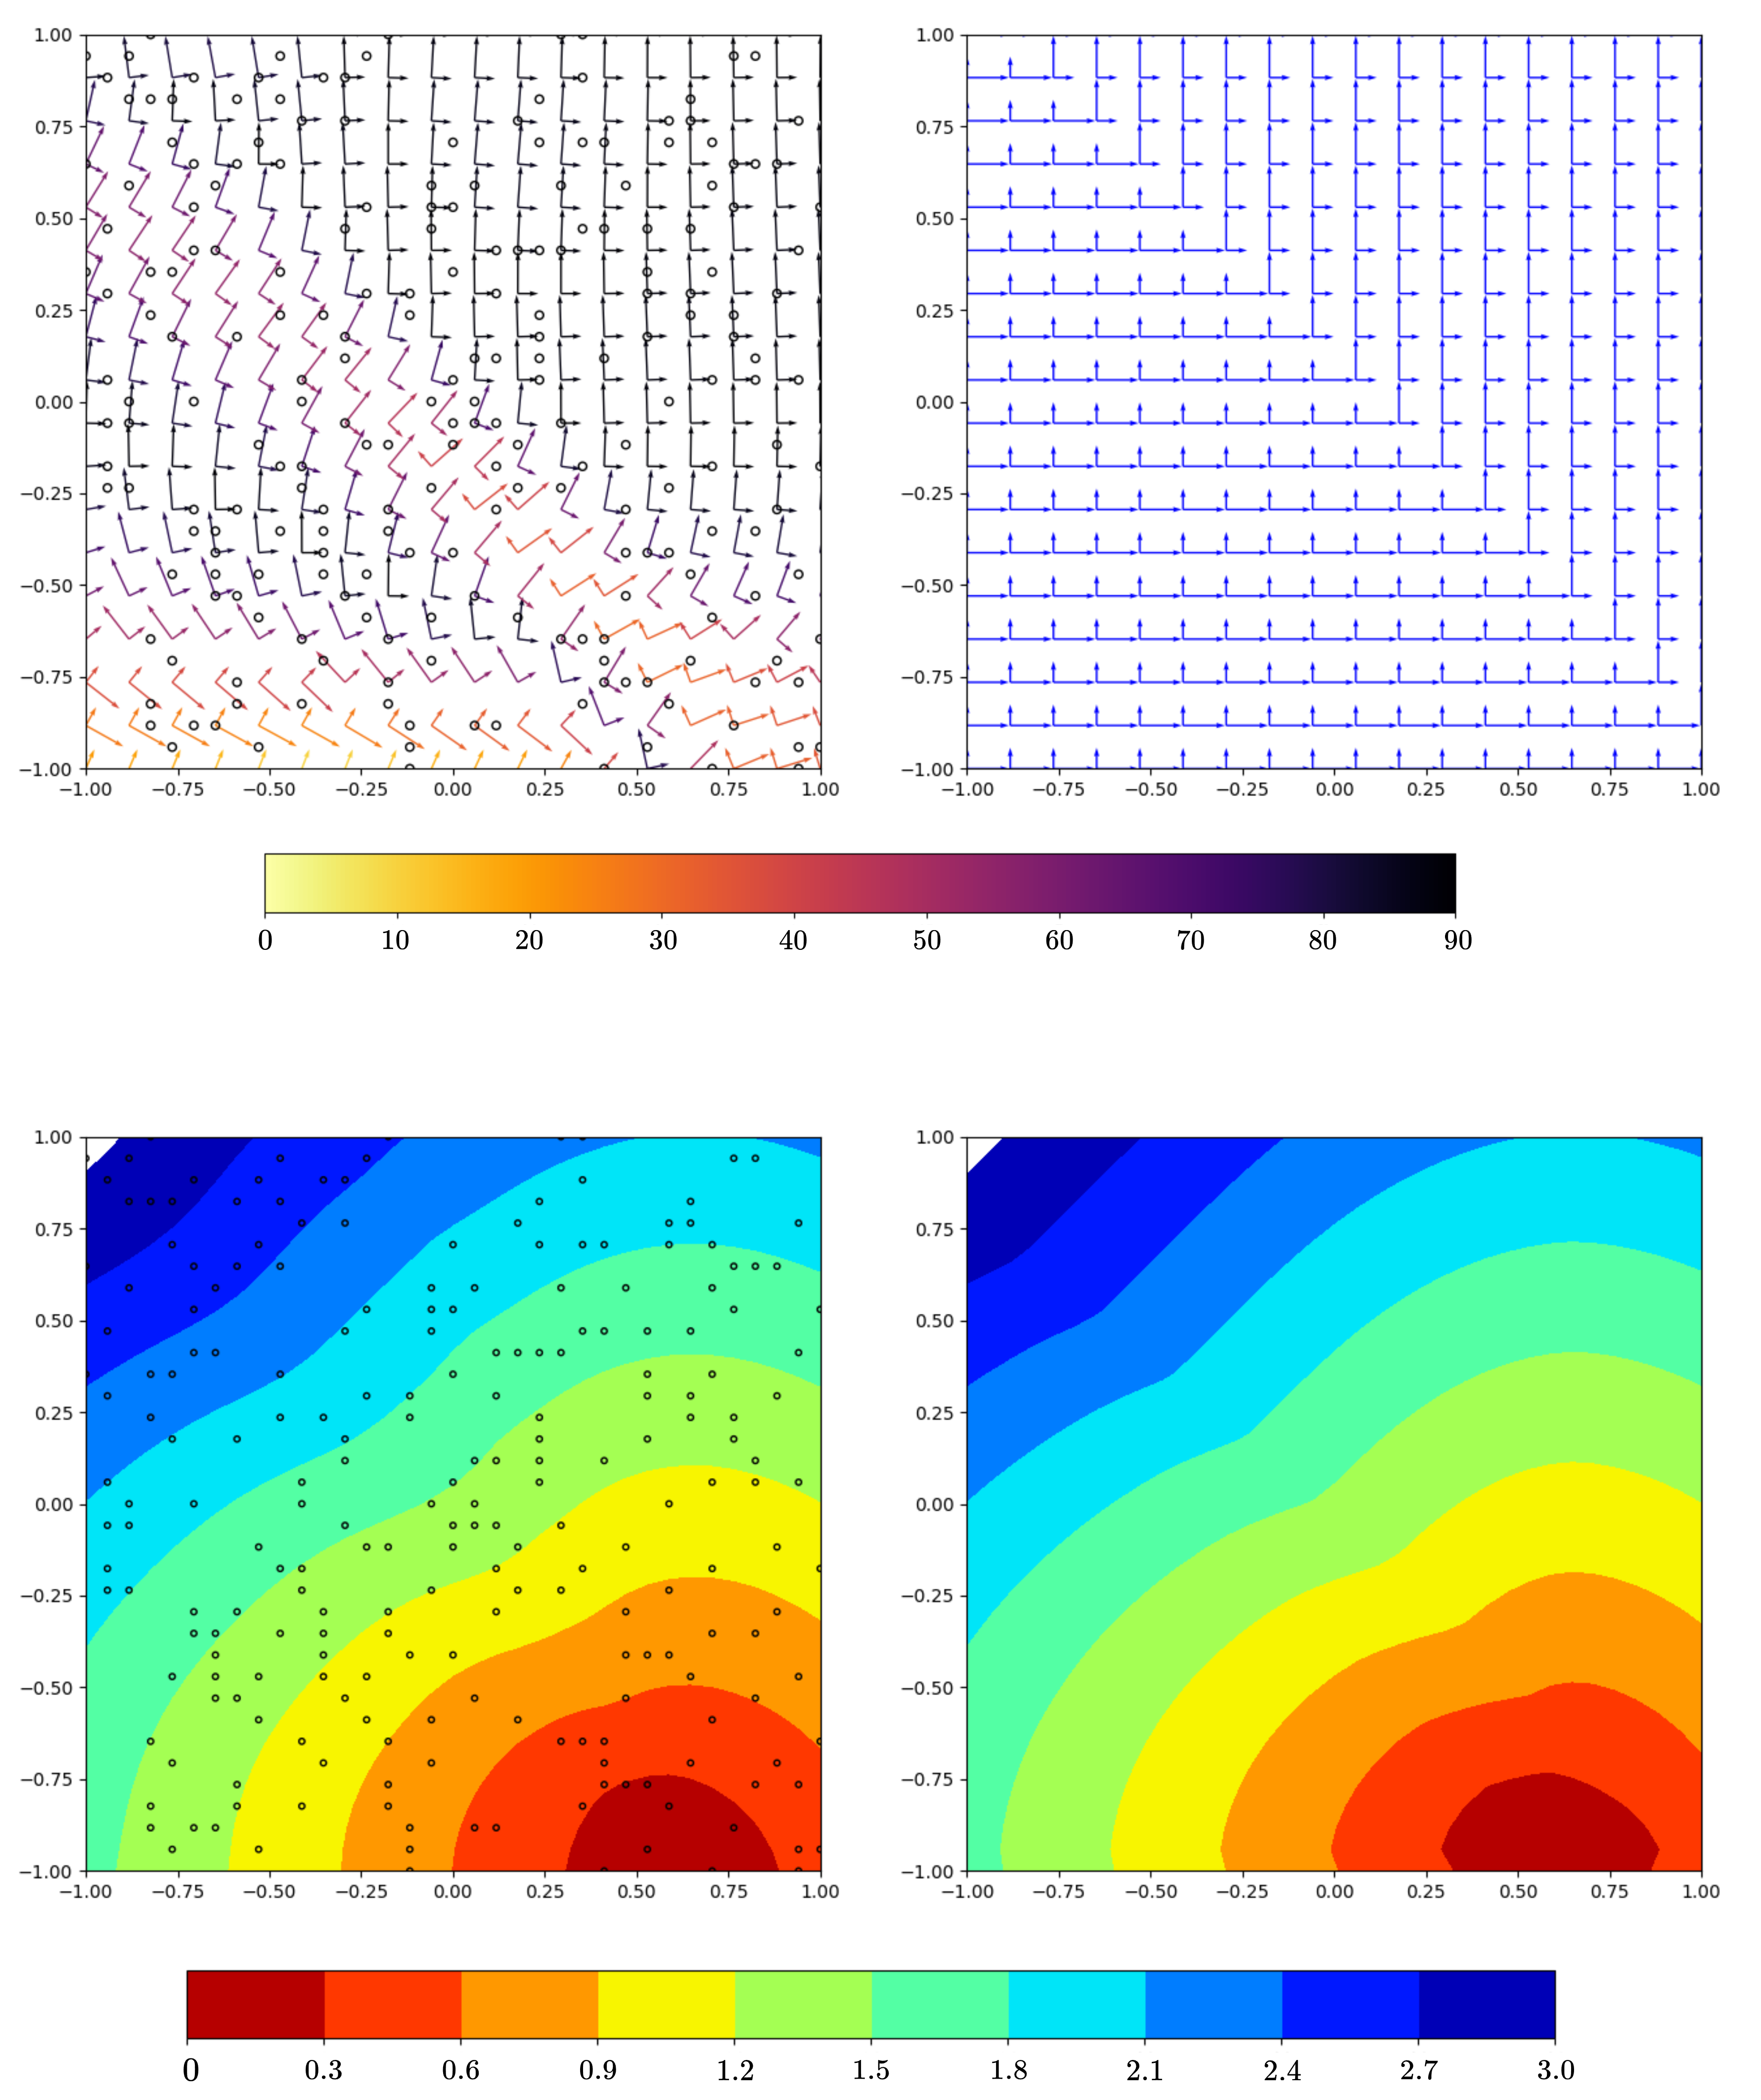
\includegraphics[width=1\linewidth]{figures/results.png}
    \caption{Results of the PINN framework for reconstructing activation time and conduction velocity tensor fields. The top row shows the conduction velocity tensor fields, while the bottom row presents the activation time maps. The left column contains the predictions from our framework, and the right column displays the corresponding ground truth solutions. The black circles indicate the spatial locations of the sampled data points.}
    \label{fig:results}
\end{figure}
We evaluated our framework on a synthetic 2D experiment. On a 35x35 grid over the domain $\Omega = [-1,1]^2$, we defined an anisotropic conduction velocity tensor field D(x, y) \cite{RuizHerrera2022}:
\begin{equation}
\mathbf{D}(x, y) =
\begin{cases}
\begin{bmatrix} 1 & 0 \\ 0 & 0.5 \end{bmatrix} & \text{if } x + y < 0, \\
\begin{bmatrix} 0.5 & 0 \\ 0 & 1 \end{bmatrix} & \text{otherwise.}
\end{cases}
\end{equation}

This piecewise configuration introduces sharp transition in conductivity properties and direction-dependent conduction, resembling the behavior observed in fibrotic or heterogeneous myocardial tissue. A ground-truth activation time map was generated by solving the anisotropic Eikonal equation using a Fast Iterative Method (FIM) \cite{Grandits2021}, with the stimulation site randomly selected via Latin hypercube sampling \cite{Stein1987}.

From the synthetic activation time map, 245 points were randomly sampled to simulate sparse catheter data. These samples served as input to the PINN framework, which aimed to reconstruct the activation time field $\phi(\mathbf{x})$ and the underlying conduction velocity tensor field $\mathbf{D}(\mathbf{x})$.

We trained the model for 3000 iterations (batch size 32) using the ADAM optimizer, with loss weights $\alpha_{\text{eiko}} = 10^{-2}$, $\alpha_{\text{reg}} = 10^{-5}$.

The PINN successfully reconstructed an activation time map closely matching the ground truth, as shown in Fig. \ref{fig:results}, with normalized root mean square error (NRMSE) of $1.76\%$. However, despite accurate wavefront recovery, the reconstructed conduction velocity tensor field showed a deviation from the true configuration, especially in regions with directional switching resulting in a mean deviation error of $24.754^\circ$.

To compare our approach, which incorporates anisotropic conduction and cardiac fiber orientation, with the isotropic method proposed by Sahli Costabal et al. \cite{SahliCostabal2020}, we used the same set of sample points as input for both frameworks. Our PINN framework achieved an NRMSE of $1.76\%$ for activation time map reconstruction, whereas the isotropic framework of Sahli et al. resulted in an NRMSE of $44.13\%$. This substantial difference highlights the importance of modeling anisotropic conduction, as the isotropic approach fails to capture the directional properties present.

To further evaluate the generalizability of our approach, we applied the framework to reconstruct multiple cardiac activation maps, each generated from distinct sampling sites simulating the catheter data. Across these experiments, the framework achieved a mean normalized root mean square error (NRMSE) of $1.67\%$ with a standard deviation of $0.51\%$, indicating robust performance in recovering activation times under varying conditions of data sparsity and sampling locations.

The framework successfully reconstructed activation times from sparse data with high accuracy, demonstrating the effectiveness of the PINN framework in capturing wavefront propagation. Regularization through Huber total variation further improved the spatial coherence of the estimated conduction tensors, promoting smoothness in the absence of dense measurements. However, the reconstruction of the full conduction velocity tensor field is still limited.   

\section{Conclusion and Future Work}

In this article, we introduced an anisotropic physics-informed neural network (PINN) framework for reconstructing cardiac activation times and direction-dependent conduction velocity tensors from sparse intracardiac catheter data. By embedding the anisotropic Eikonal equation directly into the training process, our approach models the effects of myocardial fiber orientation, an important factor often neglected by existing isotropic PINN models.

We validated our method on a synthetic 2D experiment featuring sharp conductivity transitions. The model accurately reconstructed activation maps from sparse data (RMSE: 0.0083 ms) and captured essential features of conduction anisotropy, though the reconstruction of the conduction velocity tensor field remained limited.

Despite these limitations, our results underscore the value of incorporating physiologically grounded models into neural network frameworks. This article provides a foundation for future work aimed at improving conduction velocity tensor field accuracy, and extending the approach to real 3D cardiac geometries and clinical data. Ultimately, our framework represents a promising step toward generating reliable, biophysically consistent activation maps to support catheter ablation planning and treatment of arrhythmias.

\printbibliography

\end{document}
